\section{守恒有限体积}
\label{sec:pdenum-finite-volumes}

第~\ref{chap:scalar-conservation-laws}章的激波没有导数可言，差分公式在间断处失去依据，但有一个量即使在激波处仍然成立：任意一段区间里总量的变化，等于从两端流进流出的差。有限体积方法就以这个等式为出发点。

考虑一维标量守恒律
\begin{equation}
 \partial_tu+\partial_xF(u)=0,\qquad u(x,0)=u_0(x),
 \label{eq:pdenum-conservation-law}
\end{equation}
线性输运是$F(u)=au$的特殊情形，Burgers方程是$F(u)=u^2/2$的情形。

\subsection{单元平均与通量}
\label{sec:pdenum-cell-averages}

把$x$轴分成长度$h$的单元$C_j=[x_{j-1/2},x_{j+1/2}]$，时间步长为$\tau$。把式~\eqref{eq:pdenum-conservation-law}在$C_j\times[t_k,t_{k+1}]$上积分，$\bar{u}_j(t)$是单元平均~\eqref{eq:pdenum-cell-average}，得到一个精确的关系：
\begin{equation}
 \bar{u}_j(t_{k+1})=\bar{u}_j(t_k)-\frac{1}{h}\int_{t_k}^{t_{k+1}}\bigl(F(u_{j+1/2})-F(u_{j-1/2})\bigr)\,\mathrm{d}t ,
 \label{eq:pdenum-exact-balance}
\end{equation}
其中$u_{j\pm1/2}=u(x_{j\pm1/2},t)$。这个等式对弱解也成立，它不需要$u$可导，只需要界面上的通量有意义。

式中唯一不知道的是界面上的时间积分。用仅依赖两侧单元平均的\term{数值通量}（numerical flux）$\widehat{F}$代替它，就得到\term{守恒格式}（conservative scheme）：
\begin{equation}
 U_j^{(k+1)}=U_j^{(k)}-\lambda\Bigl(\widehat{F}_{j+1/2}^{(k)}-\widehat{F}_{j-1/2}^{(k)}\Bigr),\qquad\lambda=\frac{\tau}{h},
 \label{eq:pdenum-conservative}
\end{equation}
其中$\widehat{F}_{j+1/2}^{(k)}$是在第$j$与$j+1$单元的值$U_j^{(k)},U_{j+1}^{(k)}$处算出的数值通量。数值通量\term{相容}（consistent）是指$\widehat{F}(a,a)=F(a)$，也就是在解不变的区域里通量没有偏差。

关键的结构是：单元$j$右边的通量和单元$j+1$左边的通量是同一个数。图~\ref{fig:pdenum-fv-cells}把这件事画成了账目，从一个单元流出的量恰好流进邻居。

\begin{BookInlineFigure}
 \centering
 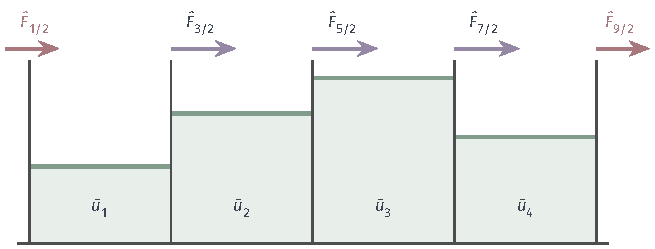
\includegraphics[width=111mm]{figures/06-differential-equations/02-partial-differential-equations/tikz/pdenum-fv-cells/figure.pdf}
 \caption{四个单元的平均值（绿）和界面通量。内部通量（紫）在左边单元中减去、在右边单元中加上，求和时抵消。总量的变化只由两端的通量（红）决定。}
 \label{fig:pdenum-fv-cells}
\end{BookInlineFigure}

把式~\eqref{eq:pdenum-conservative}对$j=1,\ldots,J$乘以$h$相加，内部的通量两两抵消，留下
\begin{equation}
 h\sum_{j=1}^JU_j^{(k+1)}=h\sum_{j=1}^JU_j^{(k)}-\tau\Bigl(\widehat{F}_{J+1/2}^{(k)}-\widehat{F}_{1/2}^{(k)}\Bigr).
 \label{eq:pdenum-telescoping}
\end{equation}
这是连续问题总量平衡的精确离散版本，不依赖$\widehat{F}$的具体形式，也不依赖$h$的大小。下面的例子说明，这个看似只是记账的性质决定了激波的速度。

\subsection{迎风与Riemann求解}
\label{sec:pdenum-upwind-riemann}

\paragraph{线性输运的迎风通量}
$F(u)=au$，设$a>0$，信息从左向右传，水流把墨水往下游带。单元界面的通量应该由上游决定，这就是\term{迎风格式}（upwind scheme）：
\begin{equation}
 \widehat{F}(U_j,U_{j+1})=aU_j .
 \label{eq:pdenum-upwind-flux}
\end{equation}
$a<0$时取$aU_{j+1}$。代入式~\eqref{eq:pdenum-conservative}，记$\mu=a\lambda$，得到更新公式
\begin{equation}
 U_j^{(k+1)}=U_j^{(k)}-\mu\bigl(U_j^{(k)}-U_{j-1}^{(k)}\bigr).
 \label{eq:pdenum-upwind}
\end{equation}

\needspace{6\baselineskip}
\paragraph{变量}
\begin{itemize}
 \item $U_j^{(k)}$：第$k$层第$j$个单元的平均，$j=1,\ldots,J$。
 \item $\widehat{F}_{j+1/2}^{(k)}$：第$j$与$j+1$单元之间的数值通量。
 \item $\mu=a\tau/h$：步长比。
\end{itemize}

\paragraph{初始化}
$U_j^{(0)}$取初值在单元上的平均。例中$a=1$，$\mu=0.5$，六个单元，方形初值的单元平均和左边界的入流状态是
\[
 \bm{U}^{(0)}=(0,\,1,\,1,\,0,\,0,\,0)^\top,\qquad U_{\text{入流}}=0 .
\]

\needspace{6\baselineskip}
\paragraph{每轮更新}
对每一层执行两步，走到$k\tau=T$结束。
\begin{enumerate}
 \item 由式~\eqref{eq:pdenum-upwind-flux}算出全部界面通量。例中第一轮，七个界面上的通量从左到右是$(0,0,1,1,0,0,0)$。
 \item 由式~\eqref{eq:pdenum-conservative}更新每个单元。例中前三轮的结果为
 \[
  \begin{aligned}
  \bm{U}^{(1)}&=(0,\,0.5,\,1,\,0.5,\,0,\,0)^\top,\\
  \bm{U}^{(2)}&=(0,\,0.25,\,0.75,\,0.75,\,0.25,\,0)^\top,\\
  \bm{U}^{(3)}&=(0,\,0.125,\,0.5,\,0.75,\,0.5,\,0.125)^\top.
  \end{aligned}
 \]
\end{enumerate}

最终各向量的分量之和都是$2$，这是式~\eqref{eq:pdenum-telescoping}的直接结果。方波被抹平了：$\mu=0.5$时每步的更新是相邻两值的平均，它和扩散有相同的作用。

\paragraph{数值黏性}
抹平的程度可以算出来。把$u$的Taylor展开代入式~\eqref{eq:pdenum-upwind}，并用方程把时间导数换成空间导数（$\partial_t^2u\approx a^2\partial_x^2u$），误差的主项给出
\begin{equation}
 \partial_tu+a\partial_xu=\nu\,\partial_x^2u+O(h^2),\qquad\nu=\frac{ah}{2}(1-\mu).
 \label{eq:pdenum-modified-equation}
\end{equation}
迎风格式更精确地求解的是一个带黏性的方程，$\nu$称为\term{数值黏性}（numerical viscosity）。它随$h\to0$消失，$\mu=1$时恰好为零，此时更新式就是整格平移。

\begin{BookInlineFigure}
 \centering
 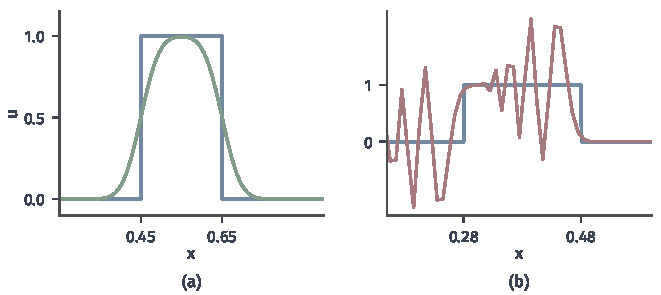
\includegraphics[width=112mm]{figures/06-differential-equations/02-partial-differential-equations/matplotlib/pdenum-upwind-smear/figure.pdf}
 \caption{$a=1$，$h=1/100$，$\mu=0.5$的方波输运。(a)$T=0.25$的迎风格式（绿）与真解（蓝），紫色虚线是修正方程~\eqref{eq:pdenum-modified-equation}的解，$\nu=0.0025$，与绿线几乎重合。(b)同样的网格用中心差分通量走到$t=0.08$（红），解已剧烈振荡。}
 \label{fig:pdenum-upwind-smear}
\end{BookInlineFigure}

图~\ref{fig:pdenum-upwind-smear}(a)中，修正方程几乎完全解释了格式的行为。(b)用的是对称的中心差分通量$\widehat{F}=a(U_j+U_{j+1})/2$，它也守恒，也相容，却不考虑信息来自哪边，第~\ref{sec:pdenum-stability}节会说明它为什么不稳定。

\paragraph{主要思想：局部Riemann问题}
Burgers方程的传播方向取决于$u$的符号，不能事先规定上游。Godunov的想法是把每个界面看作一个小的初值问题。第$k$层的单元平均是分片常数，每个界面两侧的两个常数构成一个Riemann问题，第~\ref{chap:scalar-conservation-laws}章已经解出了它的熵解。

Riemann问题的解沿界面$x=0$是一个常数，记为$u^*(U_L,U_R)$。只要各界面发出的波还没有碰到相邻界面，式~\eqref{eq:pdenum-exact-balance}中通量的时间平均就精确等于$F(u^*)$，这给出\term{Godunov格式}（Godunov scheme）的通量：
\begin{equation}
 \widehat{F}(U_L,U_R)=F\bigl(u^*(U_L,U_R)\bigr).
 \label{eq:pdenum-godunov}
\end{equation}

对凸的$F$，$u^*$可以按波的类型读出，图~\ref{fig:pdenum-riemann-fan}是两种情形。

\begin{BookInlineFigure}
 \centering
 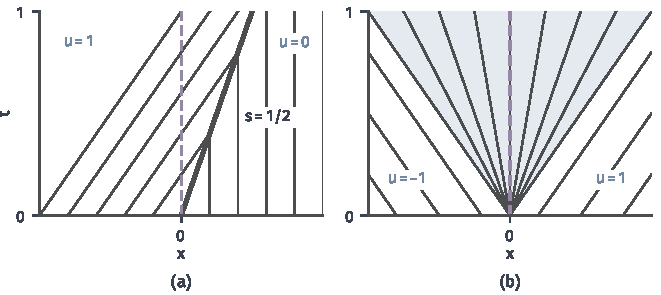
\includegraphics[width=112mm]{figures/06-differential-equations/02-partial-differential-equations/matplotlib/pdenum-riemann-fan/figure.pdf}
 \caption{Burgers方程Riemann问题的特征线（深灰），紫色虚线是界面$x=0$，Godunov通量就在这条线上读取。(a)$U_L=1$，$U_R=0$，粗线是速度$1/2$的激波，界面上的状态是$u^*=1$。(b)$U_L=-1$，$U_R=1$，浅蓝区域是稀疏波，界面上的状态是$u^*=0$。}
 \label{fig:pdenum-riemann-fan}
\end{BookInlineFigure}

$U_L\leq U_R$时解是稀疏波，$U_L>U_R$时是激波，两种情形可以合成一个公式：
\begin{equation}
 \widehat{F}(U_L,U_R)=
 \begin{cases}
 \min_{U_L\leq u\leq U_R}F(u), & U_L\leq U_R,\\
 \max_{U_R\leq u\leq U_L}F(u), & U_L>U_R .
 \end{cases}
 \label{eq:pdenum-godunov-minmax}
\end{equation}

在图~\ref{fig:pdenum-riemann-fan}(a)中，$U_L=1>U_R=0$，$u^2/2$在$[0,1]$上的最大值是$1/2$，等于$F(u^*)=F(1)$。在图(b)中，$U_L=-1<U_R=1$，$u^2/2$在$[-1,1]$上的最小值是$0$，等于$F(0)$。

\needspace{6\baselineskip}
\paragraph{变量}
\begin{itemize}
 \item $U_j^{(k)}$：第$k$层第$j$个单元的平均；$\lambda=\tau/h$。
 \item $\widehat{F}_{j+1/2}^{(k)}$：由式~\eqref{eq:pdenum-godunov-minmax}算出的界面通量。
\end{itemize}

\paragraph{初始化}
例中取Burgers方程，$\lambda=0.5$，六个单元，两端复制边界状态，也就是左边始终流入状态$1$，右边外侧始终是状态$0$：
\[
 \bm{U}^{(0)}=(1,\,1,\,1,\,0,\,0,\,0)^\top .
\]

\needspace{6\baselineskip}
\paragraph{每轮更新}
对每一层执行两步，走到$k\tau=T$结束。
\begin{enumerate}
 \item 按式~\eqref{eq:pdenum-godunov-minmax}算出全部界面通量。例中第一轮，第$3$单元及其左侧的界面通量都是$1/2$，第$3$与第$4$单元之间的状态是$(1,0)$，通量也是$1/2$，其余都是$0$。
 \item 由式~\eqref{eq:pdenum-conservative}更新。第一轮只有第$4$单元改变：
 \[
  U_4^{(1)}=0-0.5\times(0-0.5)=0.25 .
 \]
 第二轮界面$(1,0.25)$的通量仍是$1/2$，界面$(0.25,0)$的通量是$F(0.25)=0.03125$，于是
 \[
  U_4^{(2)}=0.25-0.5(0.03125-0.5)=0.4844,\qquad U_5^{(2)}=0.0156 .
 \]
 第三轮界面$(0.4844,0.0156)$的通量是$F(0.4844)=0.1173$，界面$(0.0156,0)$的通量是$0.00012$，
 \[
  \begin{gathered}
  U_4^{(3)}=0.4844+0.5(0.5-0.1173)=0.6757,\\
  U_5^{(3)}=0.0742,\qquad U_6^{(3)}=0.00006 .
  \end{gathered}
 \]
\end{enumerate}

最终各层分量之和依次是$3,\,3.25,\,3.5,\,3.75$，每步增加$\lambda\cdot\tfrac12=0.25$，也就是流入的量每步推动间断前进四分之一个单元。一个单元长$h$，一步时长$\tau$，所以间断的速度是$(h/4)/\tau=1/2$，这正是Rankine--Hugoniot条件给出的激波速度。这个速度来自式~\eqref{eq:pdenum-telescoping}，不依赖网格的细节。

\paragraph{丢掉守恒的代价}
Burgers方程的另一种写法$\partial_tu+u\partial_xu=0$在光滑解上与守恒形式等价。按它写一个迎风差分：$u\geq0$时
\[
 U_j^{(k+1)}=U_j^{(k)}-\lambda U_j^{(k)}\bigl(U_j^{(k)}-U_{j-1}^{(k)}\bigr).
\]
代入同一组初值，第$4$单元的$U_4=0$，修正项$\lambda U_4(U_4-U_3)=0$，$U_4$永远不变。数值解是定态，激波根本不动。

\begin{BookInlineFigure}
 \centering
 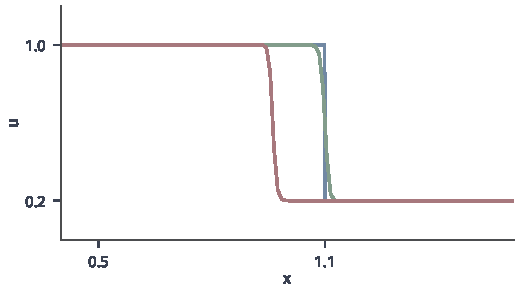
\includegraphics[width=88mm]{figures/06-differential-equations/02-partial-differential-equations/matplotlib/pdenum-godunov-shock/figure.pdf}
 \caption{Burgers方程，左状态$1$，右状态$0.2$，初始间断在$x=0.5$，$h=0.01$，$\lambda=0.5$，$T=1$。蓝线是真解，激波在$x=1.1$；绿线是Godunov格式，半高位置$1.105$；红线是非守恒的迎风差分，半高位置$0.965$，平均速度约为$0.465$，真值是$0.6$。}
 \label{fig:pdenum-godunov-shock}
\end{BookInlineFigure}

图~\ref{fig:pdenum-godunov-shock}换了一组不那么极端的数据，非守恒格式不再冻结，但速度仍然是错的。守恒的约束恰好保证了激波速度的正确，第~\ref{sec:pdenum-nonlinear}小节的定理说明这不是偶然的。

\subsection{熵选择}
\label{sec:pdenum-entropy}

守恒格式的极限若存在就是弱解，但弱解可以不唯一。第~\ref{chap:scalar-conservation-laws}章用熵条件挑出物理上的解，离散格式也需要类似的选择机制。

\paragraph{一个守恒却选错解的例子}
Godunov通量要解Riemann问题，一个省事的替代是取平均速度$s=(U_L+U_R)/2$当作波速，再按迎风法则取通量：
\begin{equation}
 \widehat{F}_{\mathrm{R}}(U_L,U_R)=
 \begin{cases}F(U_L), & s\geq0,\\F(U_R), & s<0.\end{cases}
 \label{eq:pdenum-roe}
\end{equation}
这是一种Roe型通量，它相容，代入式~\eqref{eq:pdenum-conservative}后也是守恒的。

取Burgers方程，初值在原点由$-1$跳到$1$。这时$s=0$，通量$\widehat{F}_{\mathrm{R}}=F(-1)=1/2$，它和两侧单元内部的通量相同，更新量为零。这个间断永远不动，是一个定态的膨胀激波。

它满足Rankine--Hugoniot条件，确实是弱解，只是不满足熵条件，真解是从原点展开的稀疏波。用Godunov通量走一步，$\lambda=0.5$，四个单元$(-1,-1,1,1)$的中间界面通量是$\min_{[-1,1]}F=0$，得到
\[
 U_2^{(1)}=-0.75,\qquad U_3^{(1)}=0.75,
\]
间断立即开始展开。

\begin{BookInlineFigure}
 \centering
 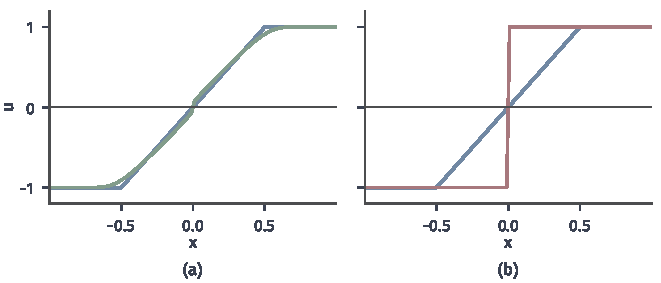
\includegraphics[width=112mm]{figures/06-differential-equations/02-partial-differential-equations/matplotlib/pdenum-entropy-fix/figure.pdf}
 \caption{Burgers方程，初值在$x=0$处由$-1$跳到$1$，$h=0.02$，$\lambda=0.5$，$T=0.5$，蓝线是熵解。(a)Godunov格式（绿）贴合稀疏波，$L^1$误差$0.047$。(b)Roe型通量（红）停留在初始的膨胀激波上，$L^1$误差$0.5$，加密网格不能改善。}
 \label{fig:pdenum-entropy-fix}
\end{BookInlineFigure}

图~\ref{fig:pdenum-entropy-fix}表明，离散守恒只负责总量，不能排除错误的间断。Roe型通量的问题出在特征速度于$U_L$和$U_R$之间变号的界面上，式~\eqref{eq:pdenum-roe}只看到了平均速度。

\paragraph{单调格式}
要选出正确的解，一个充分的结构性条件是单调。把式~\eqref{eq:pdenum-conservative}写成
\begin{equation}
 U_j^{(k+1)}=H\bigl(U_{j-1}^{(k)},U_j^{(k)},U_{j+1}^{(k)}\bigr).
 \label{eq:pdenum-scheme-h}
\end{equation}
若$H$对三个自变量都单调不减，称格式是\term{单调格式}（monotone scheme）。直观上，初值处处增大，下一层也处处增大，这和熵解的比较原理对应。

设$\widehat{F}$是Lipschitz的，对第一个变量不减，对第二个变量不增。$H$对第一、第三个变量的单调性由此直接得到，对中间变量$b$的单调性要求
\[
 \lambda\bigl(\partial_1\widehat{F}(b,c)-\partial_2\widehat{F}(a,b)\bigr)\leq1 .
\]

Godunov通量满足前两条。式~\eqref{eq:pdenum-godunov-minmax}中，增大$U_L$时，第一种情形的取最小值的区间缩小，最小值不减；第二种情形的取最大值的区间扩大，最大值不减。增大$U_R$的情形相反，通量不增。

步长条件也可以写得更具体。$\partial_1\widehat{F}(b,c)$只有$0$和$F'(b)$两种取值，后者只在$F'(b)>0$时出现；$\partial_2\widehat{F}(a,b)$同样只有$0$和$F'(b)$两种取值，后者只在$F'(b)<0$时出现。两者不会同时非零，所以条件成为
\begin{equation}
 \lambda\max\lvert F'\rvert\leq1 .
 \label{eq:pdenum-monotone-cfl}
\end{equation}

Roe型通量不单调。$U_L=-1$，$U_R=1$时通量是$1/2$；把$U_R$略微减小，$s<0$，通量变成$F(U_R)<1/2$。减小$U_R$反而减小了通量，方向与要求相反。

\paragraph{单调格式满足离散熵不等式}
对常数$c$，把$\max(a,c)$记作$a\vee c$，$\min(a,c)$记作$a\wedge c$。取Kružkov熵$\lvert u-c\rvert$，相应的熵通量是$\mathrm{sgn}(u-c)(F(u)-F(c))$。单调性足以产生这些熵不等式的离散版本。

\begin{theorem}[离散熵不等式]
 \label{thm:pdenum-discrete-entropy}
 设式~\eqref{eq:pdenum-scheme-h}的$H$单调不减，$\widehat{F}$相容。对任意常数$c$，令
 \begin{equation}
  Q_c(a,b)=\widehat{F}(a\vee c,\,b\vee c)-\widehat{F}(a\wedge c,\,b\wedge c).
  \label{eq:pdenum-entropy-flux}
 \end{equation}
 则格式的解满足
 \begin{equation}
  \begin{aligned}
  \lvert U_j^{(k+1)}-c\rvert\leq{}&\lvert U_j^{(k)}-c\rvert\\
  &-\lambda\Bigl(Q_c\bigl(U_j^{(k)},U_{j+1}^{(k)}\bigr)-Q_c\bigl(U_{j-1}^{(k)},U_j^{(k)}\bigr)\Bigr).
  \end{aligned}
  \label{eq:pdenum-discrete-entropy}
 \end{equation}
\end{theorem}

\begin{proof}
 记$a=U_{j-1}^{(k)}$，$b=U_j^{(k)}$，$d=U_{j+1}^{(k)}$。由相容性，常数状态不变，$H(c,c,c)=c$。

 由单调性，$H(a\vee c,b\vee c,d\vee c)$同时不小于$H(a,b,d)$和$H(c,c,c)=c$，所以
 \[
  H(a\vee c,b\vee c,d\vee c)\geq U_j^{(k+1)}\vee c .
 \]
 同理，
 \[
  H(a\wedge c,b\wedge c,d\wedge c)\leq U_j^{(k+1)}\wedge c .
 \]

 两式相减，并用$\lvert s-c\rvert=s\vee c-s\wedge c$，得到
 \[
  \lvert U_j^{(k+1)}-c\rvert\leq H(a\vee c,b\vee c,d\vee c)-H(a\wedge c,b\wedge c,d\wedge c) .
 \]
 代入$H$的定义，$(b\vee c)-(b\wedge c)=\lvert b-c\rvert$，通量部分合起来就是式~\eqref{eq:pdenum-entropy-flux}的差分。
\end{proof}

由相容性，$Q_c(a,a)=\mathrm{sgn}(a-c)(F(a)-F(c))$，所以$Q_c$是连续熵通量的相容逼近。这个不等式怎样传到极限，留到第~\ref{sec:pdenum-nonlinear}小节。

单调性有代价。单调格式至多是一阶精度，证明要分析格式在光滑解上的修正方程，篇幅较长，读者可查阅Harten、Hyman和Lax的原始工作。这就是单调格式总带有数值黏性的原因。
